% cmd: clear; latex graphics.tex
% cmd: clear; xdvi graphics.dvi


\documentclass{article}
\usepackage{amsmath}
%\usepackage{assymb}
\usepackage{graphicx}

\begin{document}
\title{images}
\author{Bhishan Poudel}
\maketitle
%use .PNG images whenever possible
%save the images in same directory
Here is a graph of the function
$f(x,y) = \sin\sqrt{x^2 + y^2} $

%\begin{center}

%\includegraphics[scale = 0.75]{graph.eps}
%\end {center}

\DeclareGraphicsExtensions{.pdf,.png,.jpg,.eps,.ps}
\includegraphics*[100,100][300,300]{graph}




\end {document}

%        h (here) - same location
%    t (top) - top of page
%    b (bottom) - bottom of page
%    p (page) - on an extra page
%    ! (override) - will force the specified location

%        Use the graphicx package and figure
%         environment to embed pictures
%    Pictures will be numbered automatically
%    
%    Change the width of your image by using
%     \includegraphics[width=\linewidth]{}
%    Refer to pictures in your document by
%     setting a \label and using the \ref tag
%    Set the position of your image by adding
%     a float option such as [h!]
%     
     
